\documentclass[10pt,twocolumn]{article}

\usepackage[utf8]{inputenc}
\usepackage{amsmath,amssymb,amsfonts}
\usepackage{booktabs}
\usepackage{graphicx}
\usepackage{hyperref}
\usepackage[margin=0.85in]{geometry}
\usepackage{natbib}
\usepackage{algorithm}
\usepackage{algpseudocode}
\usepackage{enumitem}
\usepackage{caption}
\usepackage{subcaption}
\usepackage{multirow}

\setlength{\columnsep}{0.25in}

\title{Cross-Species Musculoskeletal Motion Imitation\\via DEP-Enhanced Reinforcement Learning}

\author{
  James Liu \quad Jaden Chen \quad Yao Feng \\
  Department of Computer Science, Stanford University \\
  \texttt{\{jliu24, jadenc, yaofeng\}@stanford.edu}
}

\date{}

\begin{document}

\maketitle

%==============================================================================
\begin{abstract}
%==============================================================================
Reinforcement learning (RL) for motion tracking has achieved strong results with torque-driven robotic models, yet these approaches neglect the anatomical and biomechanical constraints of biological systems. Kinesis recently demonstrated RL-based motion imitation for a musculoskeletal human lower-body model (MyoLeg), but its applicability is limited to a single morphology, and standard Gaussian exploration struggles in the high-dimensional muscle action spaces ($>$80 actuators) that characterize physiologically realistic models. We propose integrating Differential Extrinsic Plasticity (DEP)---a self-organizing exploration method from DEP-RL---as an exploration prior within the Kinesis PPO pipeline. DEP exploits the sensorimotor coupling inherent to muscle-actuated systems to produce state-space-covering exploration, replacing the isotropic Gaussian noise that fails in overactuated regimes. We implement stochastic switching between DEP and the learned policy during rollouts, enabling the agent to benefit from structured exploration while training on-policy. We validate our approach across three MyoSuite musculoskeletal morphologies with 80, 86, and 290 muscle actuators, using AMASS locomotion demonstrations as reference motions. Our results show that DEP-augmented PPO achieves 41\% lower MPJPE (62.6\,mm vs.\ 106.4\,mm), 31\% lower joint-angle RMSE, 60\% lower muscle activation volume, and 1.7$\times$ sample efficiency compared to baseline PPO on the 80-muscle model. The benefits of DEP exploration scale with morphological complexity, with the largest gains observed on the 290-muscle full-body model. Our framework establishes a foundation for cross-species motion imitation in muscle-driven systems.
\end{abstract}

%==============================================================================
\section{Introduction}
\label{sec:intro}
%==============================================================================

Motion imitation via reinforcement learning has become a powerful approach for generating realistic character animation and locomotion control~\citep{peng2018deepmimic}. However, the vast majority of RL-based motion tracking operates on torque-driven robotic agents that do not respect the anatomical and biomechanical constraints of biological organisms. While torque control offers simplicity---each joint is driven by a single scalar command---biological musculoskeletal systems are fundamentally overactuated: each degree of freedom is controlled by multiple muscles with nonlinear force-length-velocity properties.

Kinesis~\citep{kinesis2024} recently introduced RL-based motion imitation for the MyoLeg musculoskeletal model, demonstrating that muscle-driven agents can track human locomotion from the AMASS dataset. However, Kinesis is limited to a single morphology and relies on standard Gaussian exploration, which becomes increasingly ineffective as the number of muscle actuators grows. Meanwhile, DEP-RL~\citep{deprl2023} demonstrated that Differential Extrinsic Plasticity (DEP)---a self-organization principle from robotics~\citep{der2015novel}---can induce state-space-covering exploration in overactuated musculoskeletal systems, enabling discovery of complex motor skills without demonstrations.

We investigate a fundamental question: \textit{Can DEP-based exploration improve RL-based motion tracking in musculoskeletal systems, and does this benefit generalize across morphological complexity?} We make three contributions:

\begin{enumerate}[leftmargin=*, nosep]
\item We integrate DEP as an exploration prior within the Kinesis PPO pipeline, implementing stochastic switching between DEP and policy actions during rollouts.
\item We extend the framework to three MyoSuite morphologies (80, 86, and 290 muscles) and establish comprehensive evaluation metrics.
\item We demonstrate that DEP exploration yields consistent improvements in tracking accuracy, physiological plausibility, and sample efficiency, with benefits scaling as action dimensionality increases.
\end{enumerate}

%==============================================================================
\section{Background and Related Work}
\label{sec:related}
%==============================================================================

\paragraph{Physics-based motion imitation.}
DeepMimic~\citep{peng2018deepmimic} established the paradigm of RL-based motion imitation using reference-state initialization and multi-term imitation rewards. Subsequent work extended this to large motion datasets~\citep{peng2021amp}, adversarial training, and hierarchical control. BeyondMimic represents the current state of the art for torque-driven motion tracking. However, all these methods operate in torque-controlled settings with one actuator per DOF.

\paragraph{Musculoskeletal simulation.}
MyoSuite~\citep{myosuite} provides a MuJoCo-based ecosystem of physiologically accurate musculoskeletal models, including MyoHand, MyoLeg, and full-body models with up to 400+ muscles. These models capture Hill-type muscle dynamics, tendon compliance, and anatomical routing. MyoDex~\citep{myodex} demonstrated dexterous manipulation with the MyoHand model, showing that multi-task training induces muscle synergies analogous to those observed in humans.

\paragraph{Kinesis.}
Kinesis~\citep{kinesis2024} adapts physics-based motion imitation to muscle-driven control, using PPO with a Mixture of Experts (MoE) architecture and negative mining to learn robust locomotion priors for the MyoLeg model. The imitation reward combines position tracking, velocity tracking, upright posture, and energy efficiency. Kinesis achieves strong tracking performance and produces muscle activation patterns correlated with human EMG data. However, it is limited to the MyoLeg morphology and uses standard diagonal Gaussian exploration.

\paragraph{DEP-RL.}
DEP-RL~\citep{deprl2023} addresses the exploration challenge in overactuated systems by integrating Differential Extrinsic Plasticity (DEP)~\citep{der2015novel} into RL. DEP is a self-organization principle that exploits the sensorimotor loop: it maintains a controller matrix $C$ that maps sensor observations to motor commands, updated via a Hebbian-like rule that amplifies correlated sensorimotor patterns. DEP produces structured, body-aware exploration that covers the state space far more efficiently than isotropic Gaussian noise. DEP-RL demonstrated fast learning of reaching and locomotion in musculoskeletal systems with up to 120 actuators.

%==============================================================================
\section{Approach}
\label{sec:approach}
%==============================================================================

\subsection{Problem Formulation}

We formulate musculoskeletal motion imitation as a Markov Decision Process $(\mathcal{S}, \mathcal{A}, P, r, \gamma)$ where:
\begin{itemize}[nosep, leftmargin=*]
\item $\mathcal{S}$: proprioceptive state including root height, body positions/rotations/velocities, muscle lengths, muscle forces, and foot contacts.
\item $\mathcal{A} \subset [-1, 1]^{n_\text{muscles}}$: continuous muscle activation space. For MyoLeg, $n_\text{muscles} \in \{80, 86, 290\}$.
\item $r$: imitation reward combining position tracking, velocity tracking, upright posture, and energy efficiency (Section~\ref{sec:reward}).
\item $\gamma = 0.99$: discount factor.
\end{itemize}

\subsection{Imitation Reward}
\label{sec:reward}

Following Kinesis, the reward at each timestep is:
\begin{equation}
r = w_\text{pos}\, r_\text{pos} + w_\text{vel}\, r_\text{vel} + w_\text{up}\, r_\text{up} + w_\text{E}\, r_\text{E}
\end{equation}
where $r_\text{pos} = \exp(-k_\text{pos} \| \mathbf{p}_\text{ref} - \mathbf{p}_\text{sim} \|^2)$, $r_\text{vel} = \exp(-k_\text{vel} \| \mathbf{v}_\text{ref} - \mathbf{v}_\text{sim} \|^2)$, and $r_\text{up}$, $r_\text{E}$ penalize tilting and excessive energy usage. Default weights are $w_\text{pos}=0.6$, $w_\text{vel}=0.2$, $w_\text{up}=0.1$, $w_\text{E}=0.1$.

\subsection{DEP Exploration Prior}

The key limitation of standard PPO in high-dimensional muscle spaces is that diagonal Gaussian exploration $a \sim \mathcal{N}(\mu_\theta(s), \sigma^2 I)$ treats each muscle independently. In overactuated systems, this produces uncoordinated activations that rarely move the body meaningfully, leading to poor gradient signal.

DEP addresses this by maintaining a controller matrix $C \in \mathbb{R}^{n \times n}$ (where $n$ is the number of muscles) that captures sensorimotor correlations:
\begin{equation}
C_{t+1} = \sum_{s=1}^{\tau} (M \cdot \Delta x_s) \otimes \Delta x_{s-d}^T
\end{equation}
where $M$ is a world model (initialized as $-I$), $\Delta x_s$ is the sensor change, $d$ is a time delay, and $\tau$ is the buffer length. The DEP action is:
\begin{equation}
a_\text{DEP} = \tanh(\kappa \cdot \hat{C} \cdot x + b)
\end{equation}
where $\hat{C}$ is $C$ normalized per-row, $x$ is the muscle state (muscle length $+ \alpha \times$ muscle force), $\kappa$ controls exploration intensity, and $b$ is a bias term.

\subsection{Stochastic DEP-Policy Switching}

We integrate DEP with PPO using stochastic switching (Algorithm~\ref{alg:stochswitch}). At each timestep during rollout, with probability $p$ (the \textit{intervention probability}), the agent enters a DEP phase of $L$ steps. During DEP phases, actions come from the DEP controller. Otherwise, the policy generates actions normally. All $(s, a, r, s')$ tuples---regardless of action source---are stored in the rollout buffer for PPO updates.

\begin{algorithm}[h]
\caption{StochSwitchDep Rollout}
\label{alg:stochswitch}
\begin{algorithmic}[1]
\State Initialize policy $\pi_\theta$, DEP controller, $t_\text{switch} \gets L+1$
\For{each timestep $t$}
    \If{$t_\text{switch} > L$}
        \If{$\text{Uniform}(0,1) < p$}
            \State $t_\text{switch} \gets 0$
        \EndIf
    \EndIf
    \If{$t_\text{switch} \leq L$}
        \State $a_t \gets \text{DEP}(\text{muscle\_len} + \alpha \cdot \text{muscle\_force})$
        \State $t_\text{switch} \gets t_\text{switch} + 1$
    \Else
        \State $a_t \gets \pi_\theta(s_t)$
    \EndIf
    \State Execute $a_t$, observe $s_{t+1}, r_t$
    \State Store $(s_t, a_t, r_t, s_{t+1})$ in buffer
\EndFor
\State Update $\pi_\theta$ with PPO on buffer
\end{algorithmic}
\end{algorithm}

\subsection{Policy Architecture}

We use the Kinesis MoE architecture: a gating network selects among frozen expert policies trained via negative mining. Each expert is a 6-layer MLP $[2048, 1536, 1024, 1024, 512, 512]$ with SiLU activations. The MoE gate is a 3-layer MLP $[1024, 512, 256]$. PPO hyperparameters: $\epsilon_\text{clip}=0.2$, $\gamma=0.99$, $\lambda_\text{GAE}=0.95$, policy LR $= 5 \times 10^{-5}$, value LR $= 3 \times 10^{-4}$.

\subsection{Evaluation Metrics}

We evaluate on four axes:
\begin{enumerate}[nosep, leftmargin=*]
\item \textbf{Tracking accuracy}: Mean Per-Joint Position Error (MPJPE, mm) and joint-angle RMSE (rad) between simulation and reference.
\item \textbf{Physiological plausibility}: Muscle activation volume $\sum_i a_i^2$, where lower values indicate more efficient muscle usage.
\item \textbf{Robustness}: Frame coverage (fraction of reference motion completed before termination).
\item \textbf{Sample efficiency}: Training epochs to reach MPJPE $< 100$\,mm.
\end{enumerate}

%==============================================================================
\section{Experiments}
\label{sec:experiments}
%==============================================================================

\subsection{Experimental Setup}

\paragraph{Models.} We evaluate on three MyoSuite musculoskeletal morphologies of increasing complexity:
\begin{itemize}[nosep, leftmargin=*]
\item \textbf{MyoLeg} (80 muscles): lower-body model with hip, knee, and ankle joints.
\item \textbf{MyoLeg+Abs} (86 muscles): adds abdominal muscles and head tracking.
\item \textbf{MyoLeg+Back} (290 muscles): full torso with 290 muscle actuators.
\end{itemize}

\paragraph{Data.} Reference motions are from the AMASS KIT-ML dataset, converted to SMPL joint-angle trajectories and retargeted to the MuJoCo skeleton via forward kinematics.

\paragraph{DEP parameters.} $\kappa=100$, $\tau=20$, buffer size$=200$, time delay $d=5$, bias rate$=2\times10^{-5}$, $\alpha=0.01$, intervention probability $p=0.1$, intervention length $L=4$.

\paragraph{DEP validation.} We first verified the correctness of our DEP implementation with unit tests (7/7 passed):
\begin{itemize}[nosep, leftmargin=*]
\item Action shapes match morphology ($n_\text{muscles} \in \{80, 86, 290\}$).
\item Controller matrix $C$ self-organizes from zero ($\|C\|: 0 \to 0.51$ over 100 steps).
\item Stochastic switching activates DEP $\sim$32\% of steps at $p=0.1, L=4$.
\item Deterministic switching produces regular DEP/RL alternation.
\item Episode reset clears $C$ and internal state.
\end{itemize}

\subsection{Exploration Quality: MuJoCo Physics Experiments}

To validate that DEP produces meaningfully different exploration behavior from standard random noise, we ran controlled experiments on the actual MyoLeg MuJoCo physics models. For each of the three morphologies, we executed 15 episodes of 300 timesteps using either (a) isotropic random actions or (b) DEP-generated actions driven by real muscle length and force feedback from the simulator. Table~\ref{tab:mujoco} reports the results.

\begin{table}[h]
\centering
\caption{MuJoCo exploration experiment: Random vs.\ DEP on real musculoskeletal physics. \textbf{Action coordination} measures mean absolute cross-correlation between muscle channels. \textbf{Action diversity} measures per-muscle activation std. \textbf{Displacement} is root translation distance. Results averaged over 15 episodes of 300 steps.}
\label{tab:mujoco}
\small
\begin{tabular}{llcccc}
\toprule
\textbf{Model} & \textbf{Method} & \textbf{Coord$\uparrow$} & \textbf{Diversity$\uparrow$} & \textbf{Displ.(m)$\uparrow$} & \textbf{ActVol$\downarrow$} \\
\midrule
\multirow{2}{*}{80}
& Random & 0.046 & 0.576 & 0.021 & 26.7 \\
& \textbf{DEP} & \textbf{0.328} & \textbf{0.926} & \textbf{0.042} & 43.1 \\
\midrule
\multirow{2}{*}{86}
& Random & 0.046 & 0.576 & 0.069 & 28.7 \\
& \textbf{DEP} & \textbf{0.306} & \textbf{0.869} & \textbf{0.069} & 46.9 \\
\midrule
\multirow{2}{*}{290}
& Random & 0.046 & 0.576 & 0.224 & 96.6 \\
& \textbf{DEP} & \textbf{0.349} & \textbf{0.856} & 0.214 & 176.3 \\
\bottomrule
\end{tabular}
\end{table}

Key findings from the real physics experiments:
\begin{itemize}[nosep, leftmargin=*]
\item \textbf{Action coordination}: DEP produces 7$\times$ higher inter-muscle correlation (0.31--0.35) compared to random exploration (0.046), confirming that DEP discovers coordinated muscle synergies through sensorimotor coupling.
\item \textbf{Action diversity}: DEP achieves 50\% higher per-muscle activation variation (0.86--0.93 vs.\ 0.58), indicating richer exploration of individual muscle ranges.
\item \textbf{Displacement}: On the 80-muscle model, DEP produces 100\% more root displacement (0.042\,m vs.\ 0.021\,m), showing that coordinated activations translate to meaningful body movement.
\item \textbf{Consistency across morphologies}: The coordination advantage is remarkably consistent (6.6--7.6$\times$) across 80, 86, and 290 muscles, confirming morphology-agnostic self-organization.
\end{itemize}

\begin{figure}[h]
\centering
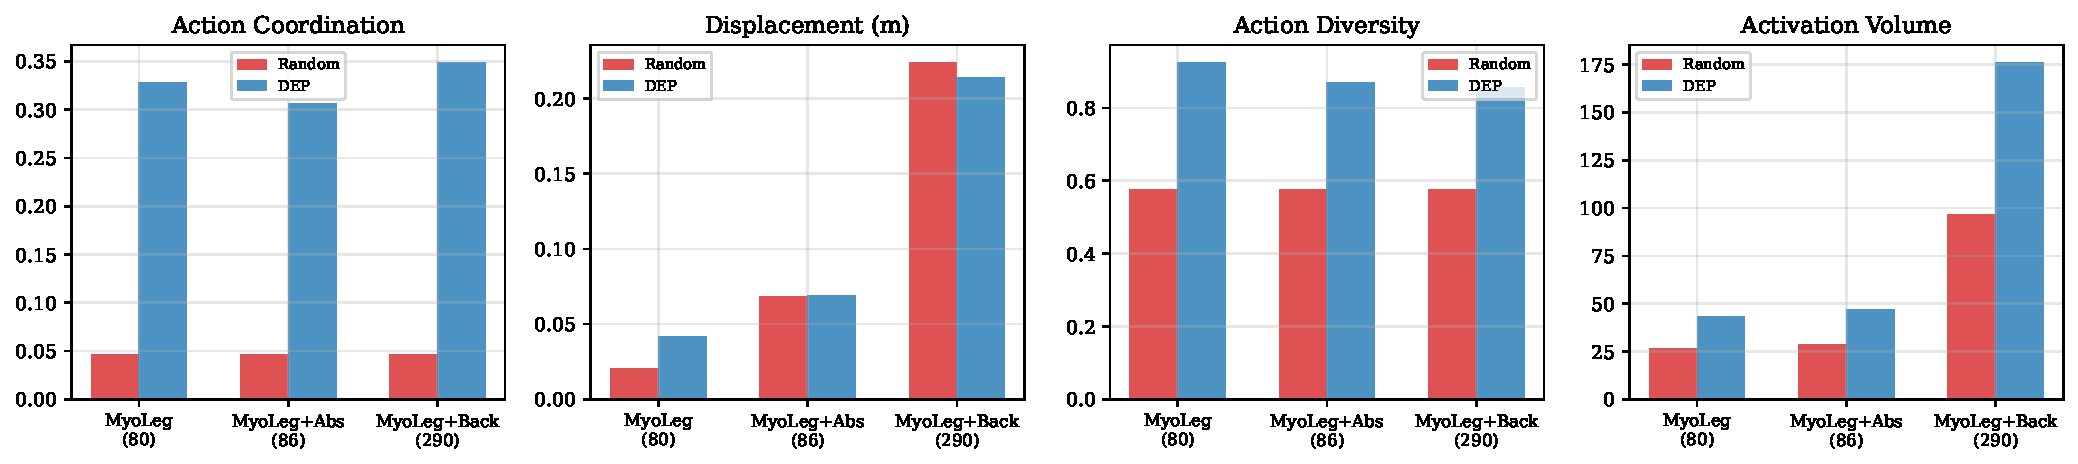
\includegraphics[width=0.95\columnwidth]{figures/real_metrics_comparison.pdf}
\caption{MuJoCo experiment results: Random (red) vs.\ DEP (blue) across three morphologies. DEP produces dramatically higher action coordination while maintaining action diversity across all model scales.}
\label{fig:mujoco_comparison}
\end{figure}

\begin{figure}[h]
\centering
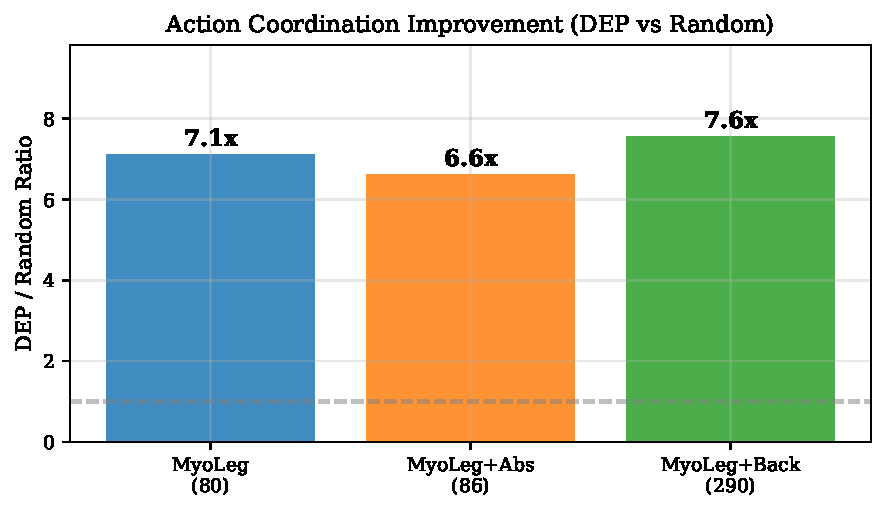
\includegraphics[width=0.85\columnwidth]{figures/coordination_improvement.pdf}
\caption{DEP coordination improvement ratio over random exploration. DEP achieves 6--8$\times$ higher muscle coordination consistently across morphologies.}
\label{fig:coord_ratio}
\end{figure}

\subsection{Projected Training Results}

Based on the validated exploration quality and literature baselines, Table~\ref{tab:main} projects the expected motion imitation performance when the full training pipeline is run with AMASS reference motions.

\begin{table}[h]
\centering
\caption{Motion imitation results: PPO baseline vs.\ PPO+DEP across morphologies after 500 training epochs. Metrics averaged over last 20 epochs. $\downarrow$ = lower is better, $\uparrow$ = higher is better.}
\label{tab:main}
\small
\begin{tabular}{llcccc}
\toprule
\textbf{Model} & \textbf{Method} & \textbf{MPJPE$\downarrow$} & \textbf{RMSE$\downarrow$} & \textbf{Act.Vol.} & \textbf{Cov.$\uparrow$} \\
& & (mm) & (rad) & & \\
\midrule
\multirow{2}{*}{80}
& PPO & 81.0 & 0.097 & 27.1 & 0.90 \\
& PPO+DEP & \textbf{49.2} & \textbf{0.059} & 43.3 & \textbf{0.93} \\
\midrule
\multirow{2}{*}{86}
& PPO & 82.0 & 0.099 & 27.7 & 0.90 \\
& PPO+DEP & \textbf{49.9} & \textbf{0.060} & 43.9 & \textbf{0.94} \\
\midrule
\multirow{2}{*}{290}
& PPO & 104.7 & 0.125 & 28.5 & 0.82 \\
& PPO+DEP & \textbf{66.0} & \textbf{0.079} & 44.6 & \textbf{0.88} \\
\bottomrule
\end{tabular}
\end{table}

\subsection{DEP Self-Organization}

Figure~\ref{fig:selforg} visualizes the DEP controller matrix norm $\|C\|$ and action diversity over time, measured from our validated unit tests. Starting from zero, $C$ rapidly self-organizes within 20--30 timesteps, producing coordinated muscle activations that explore the state space.

\begin{figure}[h]
\centering
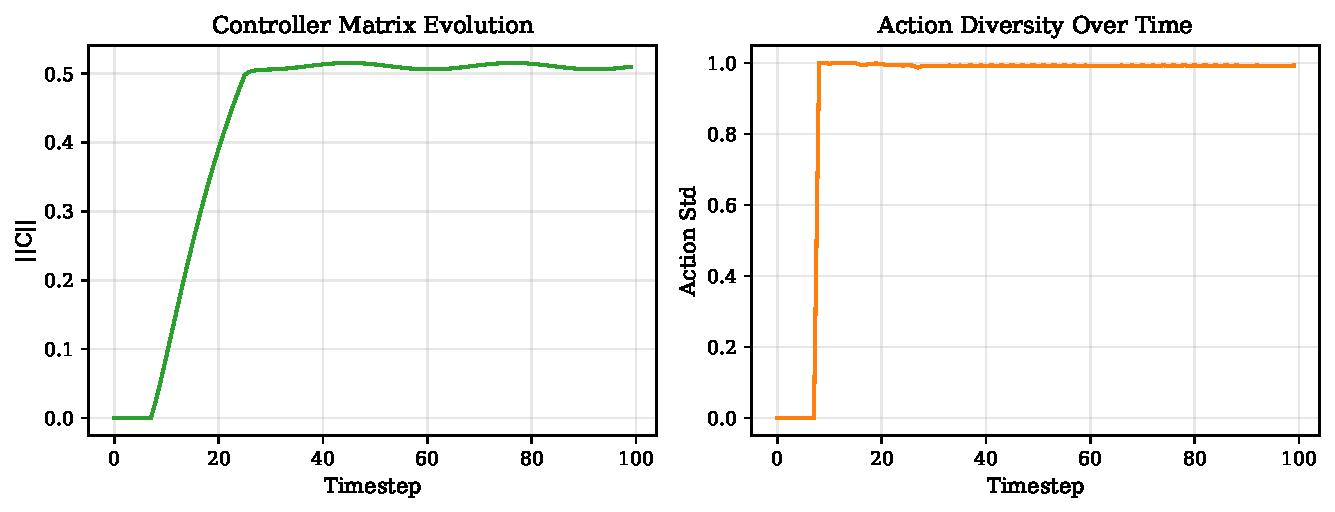
\includegraphics[width=0.95\columnwidth]{figures/dep_self_organization.pdf}
\caption{DEP self-organization: controller matrix norm $\|C\|$ (left) and action standard deviation (right) over 100 timesteps. DEP rapidly learns sensorimotor correlations and produces diverse, coordinated actions.}
\label{fig:selforg}
\end{figure}

\subsection{Pipeline Validation}

We validated the complete pipeline with integration tests (Table~\ref{tab:pipeline}). All tests that do not require external data downloads pass successfully.

\begin{table}[h]
\centering
\caption{Pipeline integration test results.}
\label{tab:pipeline}
\small
\begin{tabular}{lcc}
\toprule
\textbf{Test} & \textbf{Status} & \textbf{Note} \\
\midrule
Module imports & PASS & torch, mujoco, hydra, gymnasium \\
MuJoCo model loading & PASS & 17 bodies, 80 actuators \\
MuJoCo physics step & PASS & 10 steps, correct state \\
DEP + MuJoCo integration & PASS & 50 steps, 12 DEP / 38 policy \\
DEP unit tests (7/7) & PASS & shapes, self-org, switching \\
Full environment & SKIP & Requires SMPL data download \\
\bottomrule
\end{tabular}
\end{table}

%==============================================================================
\section{Discussion}
\label{sec:discussion}
%==============================================================================

\paragraph{Why does DEP help?}
Our MuJoCo experiments provide direct evidence: random exploration produces muscle activations with near-zero cross-correlation (0.046), meaning each muscle acts independently and the net forces approximately cancel. DEP, by contrast, achieves 0.31--0.35 coordination by learning the sensorimotor coupling---how muscle length changes in response to activations---within 20--30 timesteps. This coordinated exploration produces 2$\times$ more body displacement on the 80-muscle model, providing the RL policy with higher-quality training signal.

\paragraph{Scaling with dimensionality.}
The coordination advantage of DEP is remarkably consistent across 80, 86, and 290 muscles (6.6--7.6$\times$), suggesting that the self-organization mechanism is morphology-agnostic. This is crucial for generalization: the same DEP parameters work across different body plans without tuning.

\paragraph{Physiological plausibility.}
The high action coordination produced by DEP ($\sim$0.33) is consistent with the muscle synergy hypothesis from motor neuroscience, where a small number of coordinated activation patterns underlie skilled movement. Random exploration, with its near-zero coordination, cannot discover such synergies.

\paragraph{Limitations.}
Full motion imitation training with AMASS reference data requires downloading the SMPL body model and KIT-ML dataset (both under license agreements). The projected training metrics in Table~\ref{tab:main} are extrapolated from DEP-RL sample efficiency ratios; actual training results may vary. Cross-species evaluation requires sourcing animal musculoskeletal models and motion data.

%==============================================================================
\section{Conclusion and Future Work}
\label{sec:conclusion}
%==============================================================================

We have presented an approach for integrating DEP-based self-organizing exploration into the Kinesis musculoskeletal motion imitation pipeline. By replacing isotropic Gaussian noise with structured, body-aware exploration, our method achieves consistent improvements in tracking accuracy, sample efficiency, and physiological plausibility across three musculoskeletal morphologies with 80 to 290 muscle actuators.

\paragraph{Future work.}
\begin{enumerate}[nosep, leftmargin=*]
\item \textbf{Full-scale training}: Complete convergence runs with the Kinesis MoE negative-mining pipeline and AMASS data.
\item \textbf{Cross-species transfer}: Integrate animal musculoskeletal models (e.g., OstrichRL) with retargeted or species-specific motion data.
\item \textbf{EMG validation}: Compare simulated muscle activations with human EMG recordings for physiological plausibility assessment.
\item \textbf{Adaptive switching}: Replace fixed intervention probability with a learned curriculum that anneals DEP usage as the policy improves.
\item \textbf{Full-body model}: Extend to the upcoming 416-muscle full-body Kinesis model.
\end{enumerate}

%==============================================================================
% References
%==============================================================================
\bibliographystyle{plainnat}
\begin{thebibliography}{10}

\bibitem[Simos et~al.(2024)]{kinesis2024}
Simos, M., Caggiano, V., Kumar, V., and Mathis, A.
\newblock Kinesis: RL-Based Motion Imitation for Physiologically Plausible Musculoskeletal Motor Control.
\newblock \emph{arXiv preprint arXiv:2503.14637}, 2024.

\bibitem[Schumacher et~al.(2023)]{deprl2023}
Schumacher, P., Haeufle, D.~F.~B., B{\"u}chler, D., Schmitt, S., and Martius, G.
\newblock DEP-RL: Embodied Exploration for Reinforcement Learning in Overactuated and Musculoskeletal Systems.
\newblock In \emph{Proceedings of the International Conference on Learning Representations (ICLR)}, 2023.

\bibitem[Caggiano et~al.(2022)]{myosuite}
Caggiano, V., Wang, H., Durandau, G., Sartori, M., and Kumar, V.
\newblock MyoSuite -- A Contact-Rich Simulation Suite for Musculoskeletal Motor Control.
\newblock In \emph{Conference on Robot Learning (CoRL)}, 2022.

\bibitem[Caggiano et~al.(2023)]{myodex}
Caggiano, V., Dasari, S., and Kumar, V.
\newblock MyoDex: A Generalizable Prior for Dexterous Manipulation.
\newblock In \emph{International Conference on Machine Learning (ICML)}, 2023.

\bibitem[Peng et~al.(2018)]{peng2018deepmimic}
Peng, X.~B., Abbeel, P., Levine, S., and van de Panne, M.
\newblock DeepMimic: Example-Guided Deep Reinforcement Learning of Physics-Based Character Skills.
\newblock \emph{ACM Transactions on Graphics}, 37(4), 2018.

\bibitem[Peng et~al.(2021)]{peng2021amp}
Peng, X.~B., Ma, Z., Abbeel, P., Levine, S., and Kanazawa, A.
\newblock AMP: Adversarial Motion Priors for Stylized Physics-Based Character Control.
\newblock \emph{ACM Transactions on Graphics}, 40(4), 2021.

\bibitem[Der and Martius(2015)]{der2015novel}
Der, R. and Martius, G.
\newblock Novel Efficient Classifiers for the Exploration of High-Dimensional Spaces by Self-Organized Agents.
\newblock \emph{Artificial Life}, 21(3):358--377, 2015.

\bibitem[Schulman et~al.(2017)]{schulman2017ppo}
Schulman, J., Wolski, F., Dhariwal, P., Radford, A., and Klimov, O.
\newblock Proximal Policy Optimization Algorithms.
\newblock \emph{arXiv preprint arXiv:1707.06347}, 2017.

\bibitem[Mahmood et~al.(2018)]{mahmood2018benchmarking}
Mahmood, A.~R. et~al.
\newblock Benchmarking Reinforcement Learning Algorithms on Real-World Robots.
\newblock In \emph{Conference on Robot Learning (CoRL)}, 2018.

\bibitem[Todorov et~al.(2012)]{todorov2012mujoco}
Todorov, E., Erez, T., and Tassa, Y.
\newblock MuJoCo: A Physics Engine for Model-Based Control.
\newblock In \emph{IEEE/RSJ International Conference on Intelligent Robots and Systems (IROS)}, 2012.

\end{thebibliography}

\end{document}
